% \textit{} 斜体
% \textbf{} 粗体(使用频率应该是斜体的10%-20%)
% \ie \eg \etc
% \citet{} \citep{}

\label{sec:theory}
\begin{figure}[tb]
    \centering
    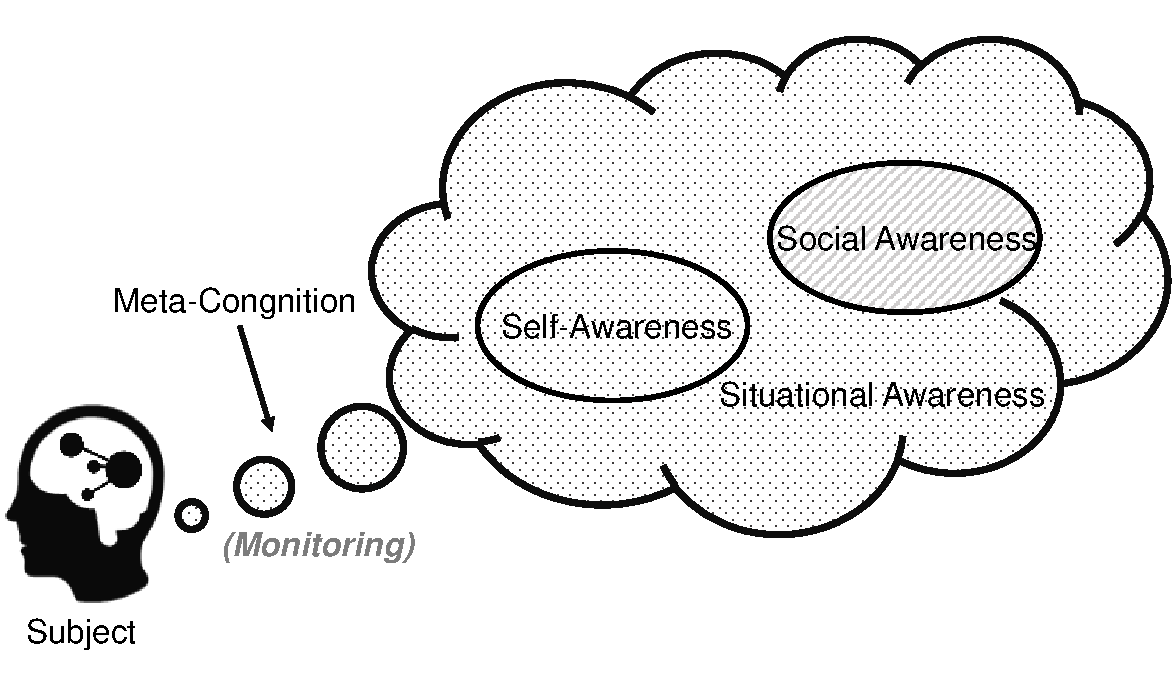
\includegraphics[width=0.85\linewidth]{Figs/four_aware.pdf} 
    \caption{\textit{Four dimensions of ``main'' awareness.} Meta-cognition monitors the subject's own processes and gives rise to self-awareness, social awareness of other individuals and the social collective, and situational awareness of the non-agent environment.}
    \label{fig:four_aware}
    \vspace{-1em}
\end{figure}

\section{Theoretical Foundations of AI Awareness}
 In this section, we will review the approaches, goals, and theories of AI consciousness that have emerged with large language models, distinguish between the research subjects that caused linguistic confusion, and clarify the targets of awareness research. In the psychology encyclopedia, awareness represents the perception or knowledge of something. When an agent possesses a ``knowledge and knowing state about an internal/external situation or fact,'' it gains awareness of its target of knowing.  Accurate reportability of something perceived or known is widely used as a behavioral index of conscious awareness. However, it is possible to be aware of something without being explicitly conscious of it \citep{apa_awareness}. Early works that navigate the range of human awareness \citep{yates1985content, turing1950mind, duval1972objective, nagel1974bat}, in which we easily conflate AI awareness with \textit{phenomenological consciousness}. In animal and human studies, consciousness represents the subjective experience of being in a certain state of mind, and having consciousness means possessing a subjective point of view \citep{nagel1974bat}. \citet{Dehaene2017} distinguish between mere global availability of information and true reflective self-consciousness, calling the latter ``C2'' or self-monitoring, which entails the system observing its own processing. To prove there is an extra layer of reflective experience, where the AI assesses its own knowledge and decisions, is difficult, if not impossible. Having a conceptual or computational self-model is not the same as having the subjective, qualitative self-awareness that humans have. Since phenomenal observations do not provide sufficient evidence for the existence of consciousness, the ``hard problem'' of AI consciousness remains scientifically unresolved \citep{nagel1974bat, chalmers2023could}. Research tends to use a theory-heavy approach to construct hypotheses for the formats of consciousness that ultimately lead to metaphysical discussions. Thus, because of the inconclusivity of metaphysical consciousness, we return to a phenomenological analysis of capacities, behaviors, and observable acquisition of knowledge.


Between 2022 and 2023, there were reports of LLMs performing tasks that required understanding the knowledge and intentions of others, abilities that are central to human social awareness. This has led to questions about whether LLMs are developing rudimentary awareness. However, it is crucial to approach these claims with care and define awareness criteria. Inspired by work in cognitive science, researchers have begun crafting definitions specific to AI. For example, \citet{berglund2023situational} define situational awareness in an AI context as the model being aware that it's a model and recognizing the difference between training/testing conditions and the real deployment environment. Separately, \citet{chen2024imitation} identify self-cognition (a term closely related to self-awareness) in LLMs as the ability of an LLM to identify its identity as an AI model (beyond just a name or role) and to demonstrate an understanding of itself. These working definitions capture the notion that an LLM with awareness would not just parrot training data blindly—it would have some internal knowledge of its own status or limits. 

\subsection{Major Types of Awareness Emergence in Modern LLMs} % Self-awareness, Situational Awareness, Social Awareness, Metacognition, Other(Goal awareness, somatic/bodily awareness)

\paragraph{Self-awareness}
 \textit{self-awareness} is a hallmark of higher consciousness, representing the ability to become the object of one's own attention and to recognize oneself as separate from others \citep{Morin2006selfawareness}. As early as 1972, \citet{duval1972objective} proposed that self-awareness states occur when an individual's attention is directed to the self as self-awareness, as opposed to the general awareness of the environment. Self-knowledge is impossible without self-awareness, and having self-awareness benefits introspection, self-regulation, and intensified emotional reactions \citep{baumeister2010self}. The self, as an apparatus that carries an individual's subjective experience, has different levels of competence. Subject's competence to be aware of themselves varies widely among animals or other intelligences who have the ability to process information, think, or give feedback to the environment to some degree, but are not always able to produce content about themselves \citep{leary2007curse, Morin2006selfawareness}. Humans learn about their identities through interacting with society, and thus, knowledge about ourselves also has social attributes and is related to emotional intelligence. \citet{eurich2018self} differentiated internal and external self-awareness among humans based on the nature of targets in the society to be aware of. Internal self-awareness represents the ability to understand the impact of one's own emotions, beliefs, states, values, and related factors on decision-making behaviors; external self-awareness represents an individual's ability to identify other individuals' perceptions of them and provide feedback on them. 
 
 Self-awareness in artificial intelligence refers to an AI system's capacity to model and understand itself as a distinct entity, including knowledge of its internal states, processes, and its relationship to the external environment. Artificial agents followed the model of humans, yet excluded several sections without strict evidence, such as emotional awareness. It represents a model's capacity to reflect on and understand its own internal states, knowledge boundaries, or behavior patterns, and recognize itself as an entity distinct from others and the environment. The components in AI self-awareness include knowledge about themselves; access to information about their own traits, characteristics, and knowledge boundaries; self-location, introspection, and self-reflection; and the ability to take an objective stance toward it as an agent in the world. Classic demonstrations include robots that can point to themselves in a mirror and AI systems that can correct their mistakes upon introspection.

\paragraph{Meta-Cognition}
\textit{Meta-cognition} was first conceptualized as ``the thinking of thinking''. \citep{flavell1979metacognition} proposed two core components of meta-cognition: metacognitive knowledge and metacognitive experiences or regulation. In the process of explaining the phenomenological consciousness and a so-called ``stage'' of being aware, \citet{Rosenthal1986-ROSTCO} also pointed out the distinction between the disposition of consciousness and the special access we have to our own mental states. Despite the abundance in the definition, with its nature of a reflective process determined, meta-cognition is gradually broken down into components: (1) self-monitoring, (2) self-reflection and probing, and (3) engagement in controlling cognitive processes \citep{efklides2001metacognitive, dunlosky2008metacognition, dunlosky2013handbook, proust2013philosophy, fleur2021metacognition}. \citet{proust2013philosophy} pointed out that meta-cognition is essentially related to an agent that is always regulating the production and distinction of cognitive processes. An agent probing its own situation constantly asks itself questions like ``Am I able to remember this information?'' and ``Will I use this module in creating the next operation?''. A regulatory module of an AI-supported automobile might be supervising its parameters and reflecting its operational status, yet without an agency or a self-probing mechanism, the module continues to run in its original setting without actively interfering, and its self-monitoring will be a result of error reporting rather than cognitive control of the primary cognitive process. In return, reflective behavior indicates at least a stimulation to a more cognitively capable agent in self-monitoring, and modern machines have the capacity to stimulate the monitoring process of reviewing their own cognitive processes.



%An LLM with meta-cognition can assess its knowledge boundary, evaluate the confidence of its answers, and adjust its reasoning strategy accordingly. Top-tier LLMs can identify which reasoning skills a task requires \citep{Didolkar2024} and even improve performance via self-reflection and iterative revision of their answers \citep{Zelikman2022, shinn2023reflexion}. The model's capacity to ``think about its own thinking'' by monitoring and regulating its cognitive processes indicates its self-evaluation and correction mechanisms --- essentially the model checking its work and refining it \citep{Walker2025}. These mechanisms have been shown to boost accuracy in complex problem-solving and code-generation tasks \citep{Didolkar2024, shinn2023reflexion}. LLMs often struggle to reliably gauge their own uncertainty or detect when they are wrong. 

\paragraph{Situational Awareness} 
SA represents the perception, comprehension, projection, and prediction of the future of the entities in the environment \citep{munir2022situational, endsley2000theoretical, nofi2000defining}. It was challenging to properly give a conclusive range of situational awareness, as with many detailed manifestations differ across psychology, engineering, and systems ergonomics \citep{sarter2017situation, nofi2000defining, stanton2010situation}. Situational awareness in LLMs typically refers to a model's understanding of its identity and the context in which it is operating. It combines the monitoring of the environment and self-locating knowledge \citep{berglund2023situational, laine2023towards,laine2024me}. Primarily, machines and models possess knowledge about facts in the environment, their own influence in the world, and their understanding of how they will be influenced by the world. When utilizing their situational awareness, agents are perceiving the world state and their own state in it in real time. In AI safety literature, this concept is often defined as an LLM being aware that it is a model and recognizing whether it is currently in a testing scenario or deployed in the real world \citep{berglund2023situational}. SA is critical because a highly capable model that knows it is being evaluated could potentially manipulate its behavior to appear aligned during tests, only to act differently once deployed. Early research has thus focused on measuring and inducing such awareness. Out-of-context reasoning evaluations show that large models can recall details about a test environment from training data (without explicit prompts) to succeed in that environment—an ability that strengthens with model size, hinting at emergent situational awareness as models scale \citep{berglund2023situational}. \citet{laine2023towards, laine2024me} performed a series of situational awareness tests and verified its importance in enhancing AI functions.  

In this article, we distinguish situational awareness from self-awareness in that the content of SA is strictly restricted to sources of information that are not directly related to the agency. From a broader perspective, an agent will naturally know that it is in the scenario modeled by LLM, and this awareness involves both self-understanding and understanding of the environment. The term is so inclusive that it overlaps significantly with self-awareness and social awareness, because any knowledge originates from an environment, and it must be gained through the agent itself. However, given the variety of shapes and purposes of machines and models, there are a number of situations in which we need to make distinctions. Collision avoidance, responsive adaptation to dynamic changes, and accurate state estimation all represent a segment of knowledge of the environment, yet the agents will not possess knowledge about themselves. For example, an autonomous car's awareness is seen in its continuous updating of a world model (other cars, lanes, pedestrians) and predicting future states to avoid. A more cognitive example is an AI security system being aware of the context (it ``knows'' that the noise it hears is the wind, not an intruder, because it integrates various sensory cues). With embodiment, sensorimotor awareness of the environment in AI can also include internal senses: a software agent might be ``aware'' of its CPU usage or memory limit as part of its situational context. In all cases, the hallmark is that the system maintains an up-to-date model of the environment and uses this model to guide immediate actions.

\paragraph{Social Awareness}

The understanding of interpersonal relationships is a basis for self-formation \citep{baumeister2010self}. Social awareness refers to the capacity to perceive and interpret the mental states, intentions, and social cues of others and respond effectively in a social context. Key components include theory of mind (understanding that others have independent beliefs and desires), perspective-taking (adopting others' viewpoints), and empathy (sharing or understanding others' emotions) \citep{Premack1978,Preston2002,Abbo2024}. By around age four, typical children pass false-belief tests, demonstrating theory of mind \citep{Wimmer1983}, whereas autistic children often fail such tasks \citep{BaronCohen1985}. Many animals also exhibit rudimentary social awareness, including primates \citep{Premack1978} and birds \citep{krupenye2019theory}. Humans further excel at shared intentionality—collaboratively understanding and aligning with others' goals and perspectives \citep{Tomasello2005}.

In artificial intelligence, social awareness can be defined as an AI system's ability to model and respond to human mental states and social cues. The AI's awareness of other agents (human or AI), their presence, state, and possibly their thoughts or intentions, constitutes its understanding of the surrounding society. This ranges from simple forms to advanced theory-of-mind reasoning. A chatbot noticing that a user is frustrated from their tone grasps an external understanding of human agents, while a robot deducing that its human partner is unaware of a certain fact and thus offering that information represents a higher level of societal understanding. Recent LLMs and chatbots have shown striking (if superficial) social-cognitive abilities: they can solve many theory-of-mind tasks and interpret indirect cues in conversation, sometimes approaching human-level performance \citep{Kosinski2024, strachan2024testing, qiu2024evaluating} and outperforming humans on certain social reasoning benchmarks, such as choosing appropriate behavior in situational judgment scenarios \citep{Mittelstaedt2024}. 

\begin{table}[htbp]
\centering
\caption{Examples of Detailed Awareness Types Mapped to Core Categories}
\label{tab:awareness-mapping}
\renewcommand{\arraystretch}{1.1} % 紧凑一点的行高
\setlength\tabcolsep{6pt}        % 缩小列间距
\begin{tabular}{@{}p{2.5cm}p{2.5cm}p{7.5cm}@{}}
\toprule
\textbf{Detailed Awareness} & \textbf{Mapped Core Category} & \textbf{Reason} \\
\midrule
Moral/Ethical Awareness 
  & Self‑awareness + Meta‑cognition 
  & Self‑awareness: knows ethical/legal constraints;\newline
    Meta‑cognition: monitors responses for ethical risks. \\

Spatial/Temporal Awareness 
  & Situational Awareness 
  & Focused perception, understanding and prediction of external space and time dynamics. \\

Emotional Awareness 
  & Social Awareness + Self‑awareness 
  & Social Awareness: perceives and responds to others’ emotions;\newline
    Self‑awareness: aware of the emotional impact of its own outputs. \\

Goal/Task Awareness 
  & Situational Awareness + Meta‑cognition 
  & Situational Awareness: understands task environment and progress;\newline
    Meta‑cognition: monitors effectiveness of strategies. \\

Safety/Risk Awareness 
  & Meta‑cognition + Self‑awareness 
  & Meta‑cognition: identifies potential errors or risks;\newline
    Self‑awareness: knows its safety/compliance boundaries. \\
\bottomrule
\end{tabular}
\end{table}


\subsection{Uncovered and Overlapping sections}
By definition, AI agents are able to acquire \emph{awareness} about any perceived object as long as they possess the ability to receive and remember information and let us realize their knowing stage. Thus, we can trivially subdivide these categories based on common sense. For instance, goal awareness represents the knowledge of why an agent is doing something. Even relatively simple AI planners have this implicitly (the goal state is defined), but an aware AI can explicitly reason about its goals (``I need to achieve X, and I am currently pursuing sub-goal Y''). A scheduling AI might say, ``I cannot schedule that meeting because I am already tasked with a higher priority deadline at that time,'' showing awareness of its hierarchy of goals. Our taxonomy, as shown in \autoref{fig:four_aware}, based on the type of object and the locus of information source (internal or external), basically encompasses objects of awareness that fit the attempt, while dispatching some parts that are difficult to identify in machines (for instance, emotional awareness).

These categories are not completely independent—they often overlap, as we show in \autoref{tab:awareness-mapping}. For example, for an AI to have social awareness, it helps if it has self-awareness (to analogize others to itself). Goal awareness and self-awareness intertwine when the AI contemplates its own goals (``I want X'' entails an ``I'' and an objective). Nonetheless, this breakdown is useful for analyzing which aspects of awareness a given AI system has. A self-driving car has excellent sensorimotor situational awareness but no self-concept beyond coordinates on a map. A dialogue agent might have some social awareness (it tracks the user's preferences) but zero embodiment or sensorimotor awareness. A research robot might have a self-model and thus self-awareness, but only rudimentary social understanding. The long-term vision in AI research is sometimes described as achieving integrated awareness: combining these types so that an AI can fluidly understand itself, its goals, its world, and others - a step toward more general forms of intelligence.

